\documentclass[smaller]{beamer}

\usepackage{helvet}
\usepackage{hyperref, graphicx}
\usepackage{amsthm}
\usepackage{amsfonts}
\usepackage{etoolbox}
\usepackage{wrapfig}
\usepackage{tikz}
\usepackage{ulem}
\usepackage{fontspec}
%\usepackage[T1]{fontenc}
%\setmainfont{Cambria}
%\usefonttheme{serif}

\usetheme{default}
\setbeamertemplate{navigation symbols}{}
\AtBeginSection[ ]
{
\begin{frame}{Outline}
    \tableofcontents[currentsection]
\end{frame}
}

% Default fixed font does not support bold face
\DeclareFixedFont{\ttb}{T1}{txtt}{bx}{n}{11} % for bold
\DeclareFixedFont{\ttm}{T1}{txtt}{m}{n}{12}  % for normal - use in headings

% Custom colors
\usepackage{color}
\definecolor{TUGray}{RGB}{101,101,137}
\definecolor{TUBlack}{RGB}{30,0,0}
\definecolor{mygreen}{RGB}{45,111,63}
\definecolor{keywords}{RGB}{205,114,0}
\definecolor{comments}{RGB}{181,51,139}
\definecolor{strings}{RGB}{58,144,81}
\definecolor{numeric}{RGB}{66,110,176}
\definecolor{linos}{rgb}{0.4,0.4,0.4}
\definecolor{links}{rgb}{0,0.4,0.75}

\definecolor{bggray}{RGB}{232, 233, 235}

\usecolortheme[named=mygreen]{structure}
\setbeamercolor{normal text}{fg=TUBlack}\usebeamercolor*{normal text}

\setbeamercolor{codecol}{fg=TUGray!25!black,bg=bggray}

\hypersetup{colorlinks, linkcolor=links, urlcolor=links}



\usepackage[sfdefault,scaled=.85]{FiraSans}
\usepackage{newtxsf}

\usepackage{listings}

\newtoggle{InString}{}% Keep track of if we are within a string
\togglefalse{InString}% Assume not initally in string

\newcommand\digitstyle{\color{numeric}}
\makeatletter
\newcommand{\ProcessDigit}[1]
{%
  \ifnum\lst@mode=\lst@Pmode\relax%
   {\digitstyle #1}%
  \else
    #1%
  \fi
}
\makeatother

\lstset{literate=%
    {0}{{{\ProcessDigit{0}}}}1
    {1}{{{\ProcessDigit{1}}}}1
    {2}{{{\ProcessDigit{2}}}}1
    {3}{{{\ProcessDigit{3}}}}1
    {4}{{{\ProcessDigit{4}}}}1
    {5}{{{\ProcessDigit{5}}}}1
    {6}{{{\ProcessDigit{6}}}}1
    {7}{{{\ProcessDigit{7}}}}1
    {8}{{{\ProcessDigit{8}}}}1
    {9}{{{\ProcessDigit{9}}}}1
	{<=}{{\(\leq\)}}1
	{>=}{{\(\geq\)}}1,
	% morestring=[b]",
    % morestring=[b]',
    % morecomment=[l]{//},
}

\lstdefinelanguage{Pseudo}{
    morekeywords={return, while, if, for, input},
    morecomment=[l]{\#},
}

% Pseudocode style
\newcommand\pseudostyle{\lstset{
language=Pseudo,
basicstyle=\fontfamily{ccr}\scriptsize,
commentstyle=\it\scriptsize\color{linos},
keywordstyle=\it\bfseries\scriptsize,
mathescape=true,
literate=
    {=}{$\leftarrow{}$}{1}
    {==}{$={}$}{1}
    {<=}{{\(\leq\)}}1
	{>=}{{\(\geq\)}}1,
xleftmargin=18pt,
xrightmargin=4pt,
aboveskip=12pt,
belowskip=0pt,
frame=tB,
keepspaces=true
}}

% Python style for highlighting
\newcommand\pythonstyle{\lstset{
language=Python,
basicstyle=\ttfamily\tiny,
numbers=left,
numberstyle=\tiny\color{linos},
morekeywords={self, np},              % Add keywords here
keywordstyle=\tiny\color{keywords},
commentstyle=\it\tiny\color{comments},    % Custom highlighting style
stringstyle=\tiny\color{strings},
xleftmargin=18pt,
xrightmargin=4pt,
aboveskip=0pt,
belowskip=0pt,
escapeinside={(*@}{@*)},
frame=l,                         % Any extra options here
showstringspaces=false,
keepspaces=true
}}

% Pseudocode environment
\lstnewenvironment{pseudo}[1][]
{
    \pseudostyle
    \lstset{
        #1
    }
}
{}

% Python environment 
\lstnewenvironment{python}[1][]
{
	\pythonstyle
	\lstset{
	#1
	}
}
{}

% wrap the Python environment
\newenvironment{codeblock}
    {\hfill\begin{beamerboxesrounded}[lower=codecol, width=0.8\textwidth]
    \medskip

    }
    { 
    \end{beamerboxesrounded}\hfill
    }

\theoremstyle{example}
\newtheorem{question}{Question}

\newcommand{\ct}[1]{\lstinline[language=Python]!#1!}
\newcommand{\ttt}[1]{{\small\texttt{#1}}}
\newcommand{\lsitem}[2]{\ttt{{#1}[}\ct{#2}\ttt{]}}

\newcommand{\x}{\textbf{x}}
\newcommand{\ix}[1]{{\it #1}}

\author{Chris Cornwell}
\date{April 14, 2025}
\title{Selecting the Machine Learning Model}

\begin{document}

\begin{frame}
\titlepage
\end{frame}

\begin{frame}
    \frametitle{Outline}
    \tableofcontents
\end{frame}

\section{Overfitting \\ Having only concern be to minimize empirical loss}

%%%%
\begin{frame}
\frametitle{Intro}
Given sample data $\mathcal S$, consisting of greyscale images of handwritten digits $0,1,\ldots,9$, say we want a decision tree model to predict the correct digit, given an image. 

Let the images be $p$ pixels by $p$ pixels. For an image, we might take the $p^2$ greyscale values (0{--}255) and lay them end to end to get a vector in $\mathbb R^{p^2}$. Then, could train a decision tree with however many splits are needed so that each leaf has points in $\mathcal S$ with only one label. 
\begin{itemize}
    \item Gives 100\% accuracy on $\mathcal S$, the data used to determine the parameters.
    \item But, the model won't perform nearly as well on data not from $\mathcal S$. 
\end{itemize}

Let's look at doing exactly this, using images of digits available from the Python package scikit-learn. 
\end{frame}

%%%%
\begin{frame}[fragile]
    \frametitle{Decision tree model for handwritten digits}
The images of digits from scikit-learn are $8$ pixels by $8$ pixels. With the submodule \ttt{datasets} imported from \ttt{sklearn}, the data can be loaded as follows.

\begin{codeblock}

\begin{python}
data = datasets.load_digits()
x = data.images
y = data.target
\end{python}

\end{codeblock}

To convert each $8\times 8$ array to a vector in $\mathbb R^{64}$, can use the \ttt{reshape} method; after assigning $\texttt{x}$ and $\texttt{y}$ as above, code below would output \ttt{(1797, 64)}.

\begin{codeblock}

\begin{python}
# make each 8x8 array into 1d array with 64 entries
x = x.reshape(len(x), -1)
x.shape
\end{python}
    
\end{codeblock}

Randomly select 20\% of the data to test model with {--} it won't be used to determine the decision tree.

\begin{codeblock}

\begin{python}
n_test = int(0.2*len(x))
test_indices = np.random.choice(len(x), size=n_test, replace=False)
train_indices = np.delete(np.arange(len(x)), test_indices)
x_test, y_test = x[test_indices], y[test_indices]
x_train, y_train = x[train_indices], y[train_indices]
\end{python}
    
\end{codeblock}
    
*\textit{Alternatively, you can use the function} \lstinline[language=Python,stringstyle=\ttfamily]{train_test_split} \textit{from the scikit-learn submodule} \lstinline[language=Python,stringstyle=\ttfamily]{model_selection}.
\end{frame}

%%%%
\begin{frame}[fragile]
    \frametitle{Decision tree model for handwritten digits}
With the setup from the last slide, use the training data to determine the decision tree.

There is a submodule \lstinline[language=Python,stringstyle=\ttfamily]{tree} within scikit-learn that we can use.

\begin{codeblock}

\begin{python}
model = tree.DecisionTreeClassifier()
model.fit(x_train, y_train)
\end{python}

\end{codeblock}

The default behavior of the \ttt{.fit()} method is that the tree has as many splits (decision stumps) as needed so that each leaf consists of points with a single label. The accuracy on \lstinline[language=Python,stringstyle=\ttfamily]{x_train} is, therefore, 100\%. 

The accuracy of the model on \lstinline[language=Python,stringstyle=\ttfamily]{x_test} will depend some on which points were put into \lstinline[language=Python,stringstyle=\ttfamily]{x_test}; however, it tends to be around only 85\%.

What happened is that the \textit{hypothesis class}, that set of functions that were possible outcomes to be the trained model, was too large (allowed too many possibilities for the resulting model). 
\end{frame}

%%%%
\begin{frame}
    \frametitle{Keeping the hypothesis class small}
We discuss a (somewhat absurd) example to demonstrate the point that 
\begin{center} small empirical loss $\not\Rightarrow$ small population loss\end{center}

\begin{wrapfigure}{r}{0.4\textwidth}
    \begin{center}
        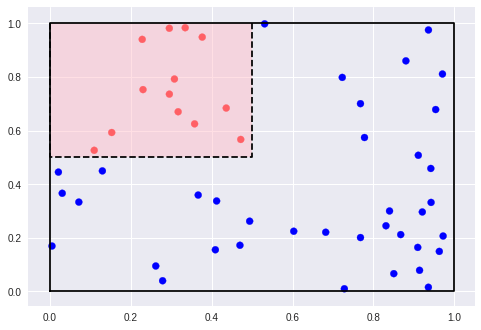
\includegraphics[width=0.38\textwidth]{../../Images/fourth_square-13v37.png}
    \end{center}
    \caption{Upper-left square labeled -1}
\end{wrapfigure}

Allowing for \textit{any} function as a possible model, for any training data $\mathcal S = \{(\x_i, \ix y_i)_{i=1}^n$, with labels in $\{1,-1\}$, we set 
        \[f_S(\x) = \begin{cases}\ix y_i,& \textrm{ if }\x = \x_i \\ 
                                    -1,& \textrm{ otherwise.}
        \end{cases}\]
Regardless of $\mathcal S$, or the population distribution that it is a sample from, the empirical loss $\mathcal L_{S}(f_S) = \frac{\#\{i:\ \ix y_i \ne f_S(\x_i)\}}{n}$ is zero.
\end{frame}


%%%%
\begin{frame}
    \frametitle{Keeping the hypothesis class small}
We discuss a (somewhat absurd) example to demonstrate the point that 
\begin{center} small empirical loss $\not\Rightarrow$ small population loss\end{center}

\begin{wrapfigure}{r}{0.4\textwidth}
    \begin{center}
        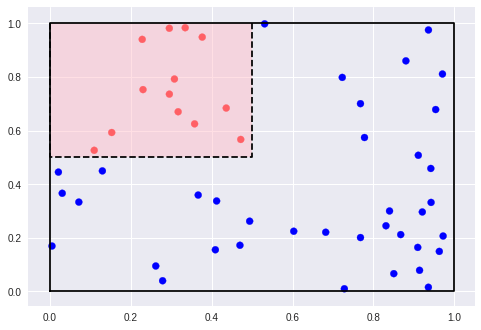
\includegraphics[width=0.38\textwidth]{../../Images/fourth_square-13v37.png}
    \end{center}
    \caption{Upper-left square labeled -1}
\end{wrapfigure}

Suppose that the population data consists of points in $[0,1]^2$ (the square of points with both coordinates between $0$ and $1$), and that a point $(x_1,x_2)$ has label $-1$ if and only if $0\le x_1 < 0.5$ and $0.5< x_2 \le 1$ (See Figure).
\vspace*{12pt}

Since a sample $\mathcal S$ is finite, a randomly chosen point has probability $0$ of being in $\mathcal S$. Thus, given a random $\x\in[0,1]^2$, with probability $3/4$ the predicted label $f_S(\x)$ is wrong.

The issue with both this model, and the decision tree that had no restriction on depth, is that the \textbf{variance} \textit{of the hypothesis class} is too large.
\end{frame}

%%%%
\begin{frame}
    \frametitle{Bias-Variance Trade-off}
    Suppose that we have chosen a hypothesis class (a class of parameterized functions, say), and a procedure that, given a training sample $\mathcal S$ from the population, determines a prediction function $f_S$.

    In order to understand the \textit{expected} population loss, we want to consider the variance of $f_S(\x)$, not only over the input space but over possible training sets $\mathcal S$. That is, over all $(\x, y)$ and $S$, the expected value $\mathbb E[(f_S(\x) - \ix y)^2]$.

    Let $\overline{h}$ be the expected prediction function, over training sets.\footnote{This takes some advanced mathematics to carefully describe. It means there is a ``measure'' on sets of functions, which allows you to integrate over a set of functions to get a new function.} In practice, you could approximate $\overline{h}$ in the following way: for samples $S_1,\ldots,S_N$, each with the same number of points, drawn i.i.d.\ from the population, then for sufficiently large $N$, 
        \[\overline{h}(\x) \approx \frac{1}{N}\sum_{i=1}^Nh_{S_i}(\x).\]
\end{frame}

%%%%
\begin{frame}
    \frametitle{Bias-Variance Trade-off}
    \begin{align*}
        \mathbb E_{S,\x, \ix y}&[(f_S(\x) - \ix y)^2] \\
            &= \mathbb E_{S,\x, \ix y}[(f_S(\x) - \overline{f}(\x) + \overline{f}(\x) - \ix y)^2] \\
            &= \mathbb E_{S,\x}[(f_S(\x) - \overline{f}(\x))^2] + \mathbb E_{\x,\ix y}[(\overline{f}(\x) - \ix y)^2] + 2\mathbb E_{S,\x,\ix y}[(f_S(\x)-\overline{f}(\x))(\overline{f}(\x) - \ix y)]
    \end{align*}
    Since $\overline{f}(\x) = \mathbb E_S[f_S(\x)]$, the last term vanishes and so
    \begin{align*}
        \mathbb E_{S,\x, \ix y}[(f_S(\x) - \ix y)^2] 
        &= \mathbb E_{S,\x}[(f_S(\x) - \overline{f}(\x))^2] + \mathbb E_{\x,\ix y}[(\overline{f}(\x) - \ix y)^2].
    \end{align*}
    A similar argument shows that 
    \begin{align*}
        \mathbb E_{\x, \ix y}[(\overline{f}(\x) - y)^2] 
        &= \mathbb E_{\x}[(\overline{f}(\x) - \overline{y}(\x))^2] + \mathbb E_{\x,\ix y}[(\overline{y}(\x) - \ix y)^2].
    \end{align*}
    And so 
    {\small
    \[\mathbb E_{S,\x, \ix y}[(f_S(\x) - \ix y)^2]  
     = \mathbb E_{S,\x}[(f_S(\x) - \overline{f}(\x))^2] + \mathbb E_{\x}[(\overline{f}(\x) - \overline{y}(\x))^2] + \mathbb E_{\x,\ix y}[(\overline{y}(\x) - \ix y)^2].\]
     \begin{flushright}{\color{blue}Variance $\uparrow$}\qquad\qquad\qquad\qquad {\color{blue}Bias$^2$ $\uparrow$}\qquad\qquad\qquad {\color{blue}Noise $\uparrow$}\qquad\quad\phantom{i} \end{flushright}
    }
\end{frame}

\end{document}